\pdfoutput=1
%
\documentclass{article}
\usepackage{frascatiphys,graphicx,subfigure,amsmath,float}
%
%
\begin{document}
%
\title{\textbf{The Fermilab Muon g-2 experiment}}
\author{
Nandita Raha, on behalf of the Muon g-2 Collaboration     \\
{\em INFN, Sezione di Roma Tor Vergata, Roma, Italy}, 
\\
%{\em Affiliation second line if needed } \\
}
\maketitle
\baselineskip=11.6pt
\begin{abstract}
The anomalous magnetic moment of the muon can be both measured and computed
to a very high precision, making it a powerful probe to test the standard model and
search for new physics. The previous measurement by the Brookhaven
E821 experiment found about three standard deviation discrepancy from the predicted value.
The Muon g-2 experiment at Fermilab will improve the precision by a factor of four
through a factor of twenty increase in statistics and a threefold reduced systematic uncertainty
with an upgraded apparatus. The experiment will also carry out an improved measurement
of the muon electric dipole moment. Construction at Fermilab is well underway. 
\end{abstract}
%
\baselineskip=14pt
%
\section{Introduction and theoretical background}
The muons magnetic moment $\vec{\mu}$ is given by, 
\begin{equation}
%\label{frequecy}
\vec{\mu} = g \frac{q} {2 m}\vec{s}
\end{equation}
where the gyromagnetic ratio $g$ of the muon is predicted to be 2 in case of
structureless spin 1/2 particle of mass m and charge q, according to Dirac theory.
Experimentally it is measured to be greater than 2. The muon anomaly 
$a_{\mu}$, given by (g-2)/2 arises due to radiative corrections (RC), which couple the
muon spin to virtual fields. These mainly include quantum electrodynamic processes
(QED), electroweak loops, hadronic vacuum polarization (HVP) etc. as shown in
Fig.\ref{fig1}.
\begin{center}
\begin{figure}[h]
\vspace{0.2 cm}
\hspace{0.5 cm}
%\includegraphics[scale=0.60]{g_2.pdf}
\includegraphics[width=2.3cm,height=3.2cm,scale=0.70]{g_2.pdf}
\includegraphics[width=2.3cm,height=3.2cm,scale=0.70]{swinger.pdf}
\vspace{-0.2 cm}
\includegraphics[width=2.3cm,height=3.2cm,scale=0.45]{eweek.pdf}
\includegraphics[width=2.3cm,height=3.2cm,scale=0.45]{QCD.pdf}
\caption{\label{fig1}The SM correction in $a_{\mu}$ from
QED, electroweak loops, HVP. }
\end{figure}
\end{center}

The leading RC from the lowest order QED process from the exchange of a virtual
photon in Fig.\ref{fig1} i.e. the ``Schwinger term'', is calculated to be $a_{\mu} = (\alpha/2\pi) =$
0.00116 \cite{schwinger}. The difference between experimental and theoretical values of $a_{\mu}$
especially at sub-ppm precision, explores new physics well above the 100 GeV scale
for many standard model extensions \cite{benn}. 


%\begin{center}
%\begin{figure}[h]
%\includegraphics[scale=0.45]{error_a.pdf}
%\includegraphics[scale=0.69]{fig2.pdf}
%\caption{\label{fig2} 
%Comparison of theoretical (left) and experimental (right) values of $a_{\mu}$.}
%\end{figure}
%\end{center}
A difference of 3.6 $\sigma$ \cite{davier} between theory and experiment, could indicate several possible
models or any new model. These new models, can be generally illustrated
using a relation discussed in \cite{ Czarnecki} in which new physics (N.P.) contributions scale as \cite{Dave} 
$\delta a_{\mu}(N.P.) =\mathcal{O}[C(N.P.)] \times ( m_{\mu}/M)^2 $ where M is the N.P. mass
scale and C is the model's coupling strength, related to any N.P. contributions to the muon
mass, $C(N.P.) \equiv (\delta m_{\mu}(N.P.)/\delta m_{\mu} )$.

\begin{figure}[H]
\centering
%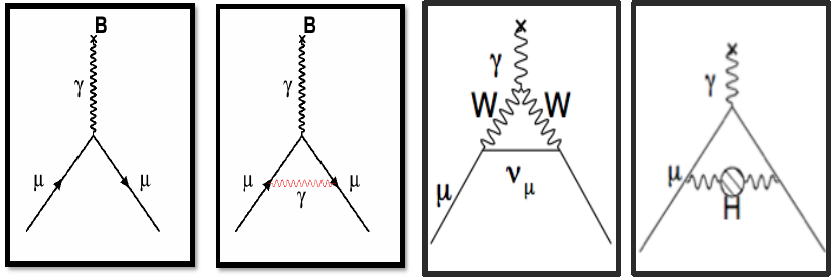
\includegraphics[width=2 cm]{a_mu_corrections.png}
\includegraphics[scale=0.2]{LM_amp.pdf}
\includegraphics[scale=0.2]{LM_time.pdf}
%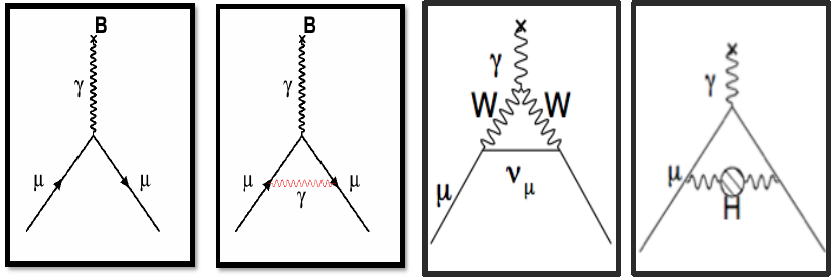
\includegraphics{a_mu_corrections.pdf}
\caption{\label{fig3}Left -- The layout of the storage ring for the E989 experiment. 
Right -- The modulated counting rate of the positron distribution of 2001 E821 data.}
\end{figure} 
In the multi-TeV scale, a muon mass is generated by radiative effects (shown in green in Fig.\ref{fig3}). 
The other possible models could be due to Z$'$, W$'$, universal extra dimensions,
littlest Higgs assume a typical weak-interaction scale coupling (shown in red in Fig.\ref{fig3}) \cite{Dave}.
The purple band in this figure represents 
unparticles, extra dimension models or SUSY with enhanced coupling \cite{Gorringe}. 
Existence of dark photons or dark $Z$ \cite{Davoudiasl:2012ig} 
%\footnote{M. Pospelov, Phys.Rev.D {\bf 80} (2009) 095002},
%\footnote{ H.~Davoudiasl, H.~S.~Lee and W.~J.~Marciano, Phys.\ Rev.\ D {\bf 86} (2012) 095009
%  doi:10.1103/PhysRevD.86.095009}
from very weakly interacting and very 
light particles would correspond to a narrow band in the 10 - 100 MeV
mass range, having an extremely small coupling, is not shown in this figure. 
In Fig.\ref{fig3} the yellow band represents the difference between theory and experiment and
the blue band represents the improvement with combined theory and experimental error.
Improved precision of measurement in $a_{\mu}$ to 140 parts per billion will continue to
constrain or validate the energy scale of the models, which is the goal of ``The E989 
Muon g-2 Experiment''. This requires 21 times more statistics than the previous
Brookhaven E821 experiment and a threefold reduction of the systematic error.
           
%Fig3 presentation
\begin{center}
\begin{figure}[h]
\hspace{1.5 cm}
%\includegraphics[width=6cm,height=3.9cm,scale=0.60]{dave.pdf}
\includegraphics[scale=0.5]{dave.pdf}
\caption{\label{fig3}
Generic classification of mass scales vs. $a_{\mu}$ contributions from new physics sources.
Various possibilities are explained in Sec.1.}
\end{figure}
\end{center}
 
\section{Storage ring technique}
A polarized muon beam (from pion decay) of energy of 3.1 GeV is injected
(through the inflector shown in Fig.\ref{fig4}) in a storage ring of uniform magnetic field of 1.45 T 
with a cyclotron frequency of $\omega_c$. Fig.\ref{fig4} shows the entire storage ring with the
kickers (K1-K3), and the quadrupoles (Q1-Q4), the collimators (C), the
NMR trolley garage and the fiber harps. An electron calorimeter is placed at
a position indicated by the calorimeter number (1 to 24).
We essentially measure the muon spin precession frequency $\omega_s$ relative to
the cyclotron frequency i.e. $\omega_a = \omega_s - \omega_c$.
\begin{center}
\begin{figure}[h!]
\hspace{2 cm}
%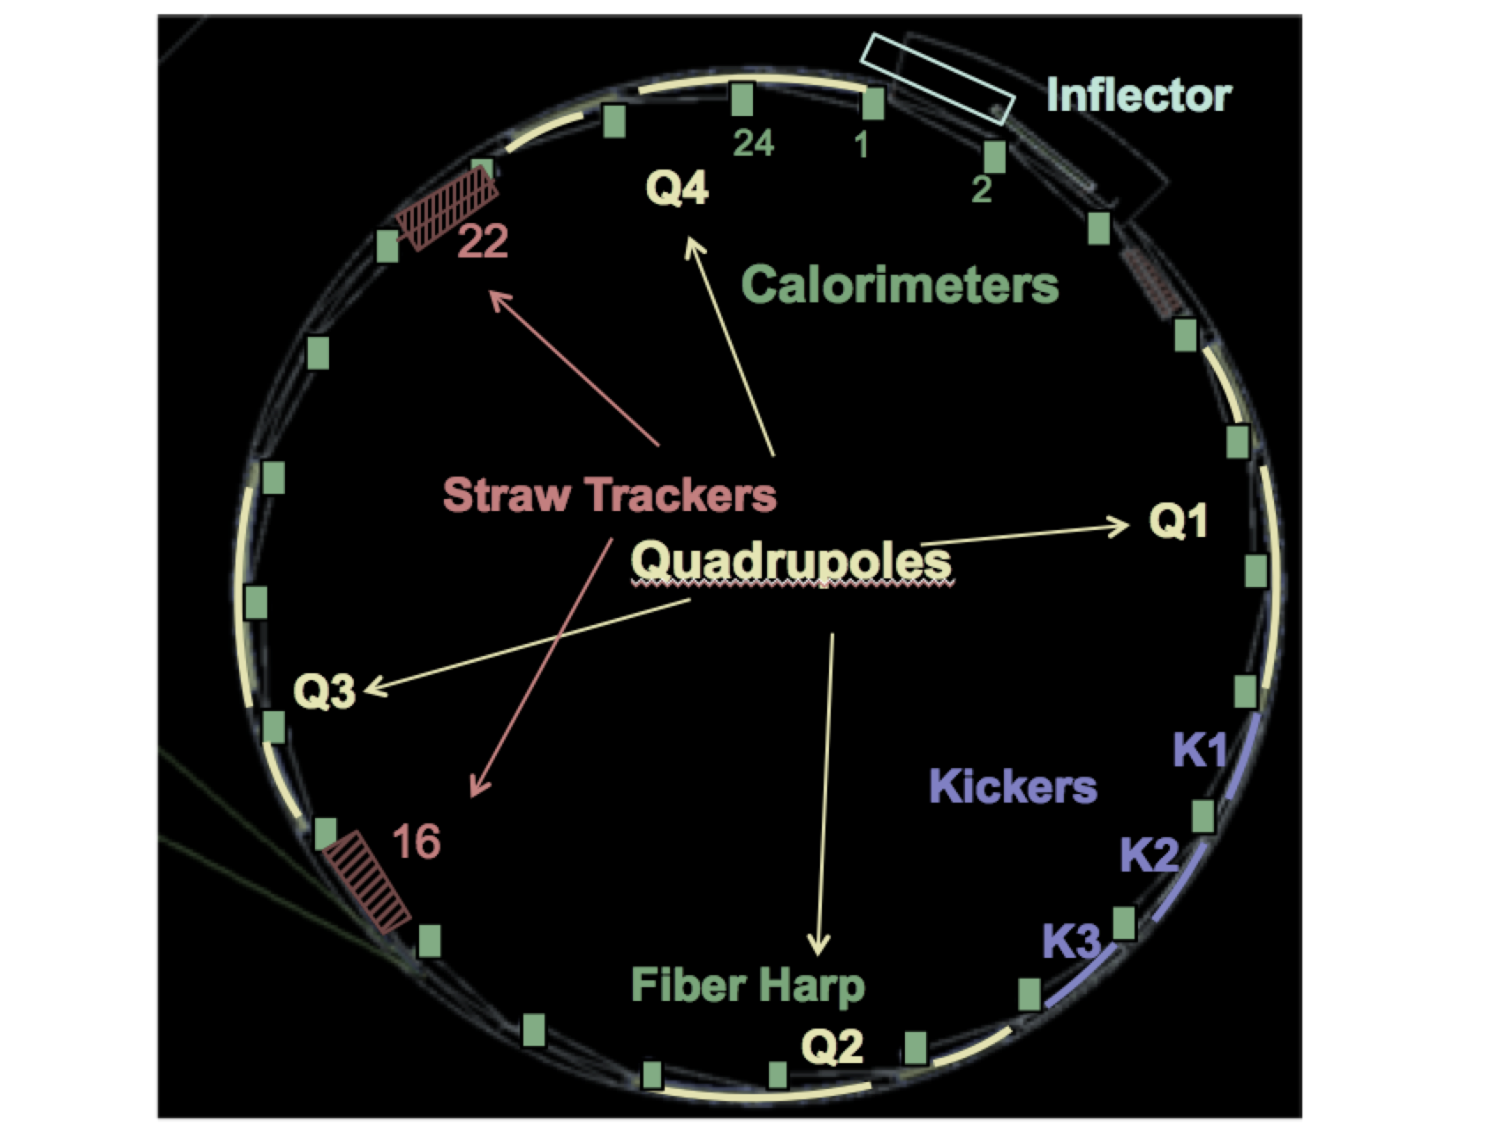
\includegraphics[width=4.5cm,height=4.5cm,scale=0.60]{ring.pdf}
\includegraphics[scale=0.50]{ring1.pdf}
\caption{\label{fig4}The layout of the storage ring from the E821 experiment.}
\end{figure}
\end{center}
These frequencies including Larmor and Thomas precession are approximately given by,
\begin{equation}
\begin{aligned}
%\mathcal{L}=\frac{g}{m}\left( \bar{L} \, \sigma_{\mu \nu} \, \ell \right)
%\partial^{\nu} \, W^{\mu} \,   + h.c. \,.
&\omega{_c} = \frac{e}{m\gamma}B\\
&\omega{_S} = \frac{e}{m\gamma}B(1 + \gamma a_{\mu})\\
&\omega{_a} = \frac{eB}{m}a{_\mu} 
\end{aligned}
\end{equation}
Thus, $a{_\mu}$ is extracted from $\omega{_a}$, provided the magnetic field B is
measured via NMR and recast $a{_\mu}$ in terms of proton precession frequency $\omega{_p}$,
\begin{equation}
\label{frequecy}
a_{\mu} = \frac{\omega{_a} / \omega{_p}}{\mu{_\mu} / \mu{_p}-\omega{_a} / \omega{_p}}
\end{equation}
 The measurement of $a_{\mu}$ also requires an accurate value of $\mu_{\mu}/\mu_p$
as seen in Eq.3. The muons decay to positrons preferentially in direction of muon spin which are
detected by the 24 calorimeters shown in Fig.\ref{fig4}. The time spectrum of these positrons is given
by,
\begin{equation}
%\label{wiggle}
N(t) = N_{0}e^{-t/\tau} (1 + A cos(\omega{_a}t))
\end{equation}
with which $\omega{_a}$ is extracted. But care needs to be taken into account
for the distortions in this spectrum due to pileup, gain instabilities, beam losses. 
\section{Experimental progress and details}
The storage ring layout is shown in Fig.\ref{fig4} of the previous section.
Here we emphasize on the details of the improvements required to achieve our goal. 
Several improvements are required to collect 21 times more
muons than the previous effort at Brookhaven E821 experiment.
This is accomplished by improved muon storage and 
using a long decay channel to produce muons that requires
improvement of existing tunnels and building 
new ones. The usage of a delivery ring to get rid of pions would 
eliminate early unwanted background. 
The improved beam structure will have 4 batches of
$4 \times 10^{12}$ protons to the Recycler in 1.33 s supercycle with a frequency of 15 Hz.
A proton batch is divided into four proton bunches of intensity $10^{12}$. Thus, the experiment
will receive 16 proton bunches per supercycle, i.e. a rate of 12 Hz.% \cite{TDR}.

We aim for enhanced improvements to the muon precession systematics due to calorimeters
and trackers. To achieve this the calorimeter should resolve multiple particles and
have high gain stability. Each calorimeter is made up of $9\times6$ PbF$_2$ Cherenkov
crystals that are read by SiPMs (Silicon Photo Multipliers) which improves the
resolution and pileup protection. 
A laser calibration system will be used 
for the accurate calibration of the calorimeters. We will develop a high-performance laser
calibration system and use it for on-line monitoring of the SiPM gain fluctuations
during the run.
This laser calibration system must have a relative accuracy at sub-per mil level to achieve the
goal of our experiment. 
The tracker should improve positron tracking (use much thinner straws) and
inform muon beam dynamics more effectively. 

We further aim for improvements to the proton precession systematics
by using new set of NMR probes and generating a more uniform magnetic
field with improved shimming of magnets.
A uniform field is essential as the signal degrades more quickly in high gradients. 
The magnetic field is measured using pulsed proton NMR with a goal of 70 ppb accuracy.
The factor of 2.4 improvement over BNL E821 will come from higher magnetic field uniformity and stability,
new lower noise NMR electronics with higher frequency resolution,
new NMR probes with higher signal to noise ratio 
and improved calibration probes and calibration techniques.
%This is accomplished using improved NMR techniques which are extremely
%precise to $\approx$70 ppb and improved shimming of magnets. 
\section{Summary}
The Muon g-2 experiment under construction at Fermilab aims for a fourfold improvement from Brookhaven E821 
in the measurement of the muon g-2. This is essential for the understanding
of QED and the Standard Model and evidence of any new physics beyond the Standard Model. 
Significant efforts in the theory of e$^+$e$^-$ measurements are also leading to an
improvement in the uncertainty in HVP along with a lot of progress on Lattice
calculations too. This will improve the theoretical calculation of g-2. Efforts 
to enhance and investigate the performance of all detector systems are taking place,
along with testing the best methods of data acquisition. We plan further installations 
in 2$^{nd}$ half of 2016 and expect data taking with muons in 2017 and initial results
in 2018. 


\section*{Acknowledgments}
This work was supported by the EU Horizon 2020 Research and Innovation Programme under the
Marie Sklodowska-Curie Grant Agreement No. 690835.
% \newpage

\begin{thebibliography}{99}
\bibitem{schwinger}
J. Schwinger, Phys. Rev. 73, 416 (1948).
  
\bibitem{benn}
G.W. Bennett, et al. Phys.Rev.D73:072003, 2006

\bibitem{davier}
Davier et al. 2011
\bibitem{Czarnecki}
A. Czarnecki and W. J. Marciano, Phys. Rev. D64,
013014 (2001)
\bibitem{Dave}
D. Hertzog, Ann. Phys (Berlin) 2015., courtesy D. Stockinger

\bibitem{Gorringe}
T. P. Gorringe and D. W. Hertzog, doi: 10.1016/j.ppnp.2015.06.001

\bibitem{Davoudiasl:2012ig}
 H.~Davoudiasl, et al. Phys.\ Rev.\ D {\bf 86} (2012) 095009


%J. Grange et al. (Muon g-2) (2015),
%1501.06858

\end{thebibliography}
%
\end{document}
